\section{Introduction}

The formation of the RoboNotts team stems from a goal to afford students practical exposure to the development of robust and dependable assistive robotics. These technologies are designed to address the challenges associated with supporting individuals in diverse scenarios, such as older adults living independently and patients in healthcare settings. The RoboNotts team operates within the Cobot Maker Space (CMS), an expressly designed area for collaborative robotics research at the University of Nottingham in Nottingham, United Kingdom, the RoboNotts team collaborates with researchers and students, serving as a dedicated testing ground for innovative research initiatives..\\

The RoboNotts team is comprised of members from a range of backgrounds, united with a common interest in robotics, and belief that assistive robotics will be an important aspect of supporting vulnerable populations in the future. The team is predominantly composed of undergraduate students from the University of Nottingham, mainly in the school of computer science, electrical engineering, and mechanical engineering. The team also includes PhD students, technicians and research associates working at the CMS. The RoboNotts team's main aim is to provide visibility to this realm of robotics, and a platform for undergraduate students to learn the skill required to thrive in robotics. \\

Structured into several specialised sub-teams, each dedicated to specific aspects of robotic development, the RoboNotts team operates under the leadership of a designated team leader. This leader assumes comprehensive responsibility for integration and oversees all organisational tasks, with support from the CMS. The team benefits from access to the 'Living Space', a designated area simulating a small flat. This space serves as an environment for the development, testing, and implementation of assistive robotics and other sensor-based systems within a home setting. The CMS has previously hosted assistive robotics competitions. 



\subsection{A Subsection Sample}
Please note that the first paragraph of a section or subsection is
not indented. The first paragraph that follows a table, figure,
equation etc. does not need an indent, either.

Subsequent paragraphs, however, are indented.

\subsubsection{Sample Heading (Third Level)} Only two levels of
headings should be numbered. Lower level headings remain unnumbered;
they are formatted as run-in headings.

\paragraph{Sample Heading (Fourth Level)}
The contribution should contain no more than four levels of
headings. Table~\ref{tab1} gives a summary of all heading levels.

\begin{table}
\caption{Table captions should be placed above the
tables.}\label{tab1}
\begin{tabular}{|l|l|l|}
\hline
Heading level &  Example & Font size and style\\
\hline
Title (centered) &  {\Large\bfseries Lecture Notes} & 14 point, bold\\
1st-level heading &  {\large\bfseries 1 Introduction} & 12 point, bold\\
2nd-level heading & {\bfseries 2.1 Printing Area} & 10 point, bold\\
3rd-level heading & {\bfseries Run-in Heading in Bold.} Text follows & 10 point, bold\\
4th-level heading & {\itshape Lowest Level Heading.} Text follows & 10 point, italic\\
\hline
\end{tabular}
\end{table}


\noindent Displayed equations are centered and set on a separate
line.
\begin{equation}
x + y = z
\end{equation}
Please try to avoid rasterized images for line-art diagrams and
schemas. Whenever possible, use vector graphics instead (see
Fig.~\ref{fig1}).

\begin{figure}
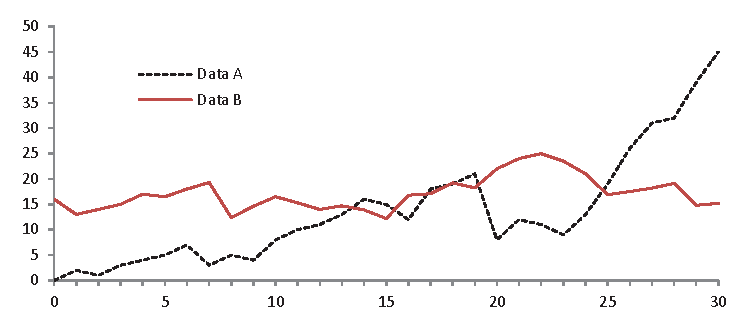
\includegraphics[width=\textwidth]{fig1.eps}
\caption{A figure caption is always placed below the illustration.
Please note that short captions are centered, while long ones are
justified by the macro package automatically.} \label{fig1}
\end{figure}

\begin{theorem}
This is a sample theorem. The run-in heading is set in bold, while
the following text appears in italics. Definitions, lemmas,
propositions, and corollaries are styled the same way.
\end{theorem}
%
% the environments 'definition', 'lemma', 'proposition', 'corollary',
% 'remark', and 'example' are defined in the LLNCS documentclass as well.
%
\begin{proof}
Proofs, examples, and remarks have the initial word in italics,
while the following text appears in normal font.
\end{proof}
For citations of references, we prefer the use of square brackets
and consecutive numbers. Citations using labels or the author/year
convention are also acceptable. The following bibliography provides
a sample reference list with entries for journal
articles~\cite{ref_article1}, an LNCS chapter~\cite{ref_lncs1}, a
book~\cite{ref_book1}, proceedings without editors~\cite{ref_proc1},
and a homepage~\cite{ref_url1}. Multiple citations are grouped
\cite{ref_article1,ref_lncs1,ref_book1},
\cite{ref_article1,ref_book1,ref_proc1,ref_url1}.